\documentclass{beamer}
\usetheme{CambridgeUS}
\usepackage{algorithm,algpseudocode}
\usepackage{lmodern, mathtools}

\title{SC2001 Project 2}
\subtitle{The Dijkstra's Algorithm}
\author[Hong, Dinh, He]{Hong Jia Yang \and Dinh Pham Minh Anh \and He Qi Xin}
\institute{Team 4}
\date{\today}

\begin{document}

\begin{frame}
	\titlepage
\end{frame}

\begin{frame}
	\frametitle{Outline}
	\tableofcontents
\end{frame}

\section{Environment Specifications}
\begin{frame}
	\frametitle{Environment}
	\begin{itemize}
		\item Software
		\begin{itemize}
			\item C++
			\item MinGW g++ 13.1.0	
			\item Header \texttt{<bits/std++.h>} 
		\end{itemize}
		\item Hardware
		\begin{itemize}
			\item OS: Windows 11 (Home) x86\_64
			\item Processor: Intel(R) Core(TM) i7-10750H (12) @ 2.59 GHz
		\end{itemize}	
	\end{itemize}
	\begin{block}{Note}
		Please refer to \texttt{JamesRobertJohns/team4project2}
	\end{block}
\end{frame}

\section{Implementation of Dijkstra's}
\subsection{Adjacency Matrix and Array}

\begin{frame}
	\frametitle{Matrix Representation of Graph}
	For a graph \( G = (V, E) \), assume that the vertices are numbered \( 1, 2, \hdots, \lvert{ V }\rvert  \) in some arbitrary manner. Then the adjacency-matrix representation of a graph G consists of a \( \lvert{ V }\rvert \times \lvert{ V }\rvert  \) matrix \( A = (a_{ij}) \) such that
	\[
		a_{ij} = \begin{cases}
			w_{ij} & \text{if } (i, j) \in E,\\
			\infty & \text{otherwise.} 
		\end{cases}
	\]

	Where \( w_{ij} \) is the weight for the weight function \( w(u, v) : E \rightarrow \mathbb{R}^+ \) 
	\onslide<2> \begin{block}{Recall}
		Dijkstra's only works for non-negative weighted Directed Graphs	
	\end{block}
\end{frame}

\begin{frame}
	\begin{columns}
	\column{0.5\textwidth}
	\begin{figure}
		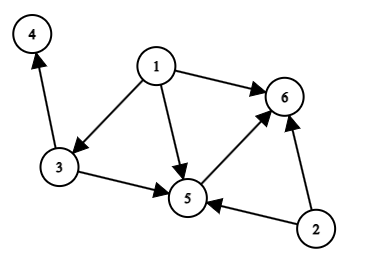
\includegraphics[scale=0.5]{./pict/exampleGraph.png}
		\caption{Graphical Example}
	\end{figure}

	\column{0.5\textwidth}
	\begin{table}
		\begin{tabular}{c|c|c|c|c|c|c}
			  & 1 & 2 & 3 & 4 & 5 & 6\\
			  \hline
			1 & $\infty$ & 1 & $\infty$ & $\infty$ & 1 & 1\\
			\hline
			2 & $\infty$ & $\infty$ & $\infty$ & $\infty$ & 1 & 1\\ 
			\hline
			3 & $\infty$ & $\infty$ & $\infty$ & 1 & 1 & $\infty$ \\
			\hline
			4 & $\infty$ & $\infty$ & $\infty$ & $\infty$ & $\infty$ & $\infty$  \\
			\hline
			5 &  $\infty$ & $\infty$ & $\infty$ & $\infty$ & $\infty$ & 1\\
			\hline
			6 & $\infty$ & $\infty$ & $\infty$ & $\infty$ & $\infty$ & $\infty$\\
			\hline
		\end{tabular}
		\caption{Matrix Representation}
	\end{table}
	\end{columns}
\end{frame}

\begin{frame}
	\frametitle{Implementation of Adjacency Matrix}
	\begin{itemize}
		\item \texttt{std::vector<std::vector<int>>} to represent the 2D array. 
		\begin{itemize}
			\item \texttt{std::vector} is a sequence container that encapsulates dynamic size arrays
			\item 0 indexed
			\item \texttt{std::numeric\_limits<int>::max()} to represent infinity
		\end{itemize}
		\item Random access: \( O(1) \) 
		\item Insertion or removal of elements at the end: \emph{amortised} \( O(1) \) 
		\item Insertion or removal of elements: \( O(n) \) 
		\item Search whether \( (u,v) \in E \): \( O(1) \) 
		\item Space Complexity: \( O(V^2) \) 
	\end{itemize}
\end{frame}

\begin{frame}
	\frametitle{Overview of Priority Queue}
	A priority queue is a data structure for maintaining a set \( S \) of elements, each with an associated value called key. The min-priority queue should support the following operations
	\begin{itemize}
		\item \texttt{INSERT(S, x)} inserts the element \( x \) into the set \( S \)\\
			\( S \leftarrow S \cup \{x\} \) 
		\item \texttt{MINIMUM(S)} returns the element of $S$ with the smallest key
		\item \texttt{EXTRACT-MIN(S)} removes and return the element of \( S \) with the smallest key
		\item \texttt{DECREASE-KEY(S, x, k)} decreases the value of element \( x \)'s key to new value \( k \), which must be at least as small as \( x \)'s current key value
	\end{itemize}
\end{frame}

\begin{frame}
	\frametitle{Naive Array Implementation} 
	\begin{columns}
	\column{0.5\textwidth}		
	\begin{itemize}
		\item Unsorted Array
		\begin{itemize}
			\item Insertion Time: \( O(1) \) 			
			\item Key Update Time: \( O(1) \) 
			\item Peek Time: \( O(n) \) 
			\item Extract Time: \( O(n) \) 
			\item Space: \( O(n) \) 
		\end{itemize}
	\end{itemize}
	
	\column{0.5\textwidth}
	\begin{itemize}
		\item Sorted Array
		\begin{itemize}
			\item Insertion Time: \( O(n) \) 
			\item Key Update Time: \( O(n) \) 
			\item Peek Time: \( O(1) \) 
			\item Extract Time: \( O(1) \) 
			\item Space: \( O(n) \) 
		\end{itemize}
	\end{itemize}
	\end{columns}
\end{frame}

\begin{frame}
	\frametitle{Sorted Array}
	\begin{algorithm}[H]
		\caption{peek at the minimum node}
		\begin{algorithmic}[1]
		\Function{minimum}{$S$}
			\State \Return $S[0]$
		\EndFunction
		\end{algorithmic}
	\end{algorithm}

	\begin{algorithm}[H]
		\caption{extract the minimum node}
		\begin{algorithmic}[1]
		\Function{extract-min}{$S$}
		\State min \( \leftarrow S[0]\) 
		\State delete $S[0]$
		\State \Return min
		\EndFunction
		\end{algorithmic}
	\end{algorithm}
\end{frame}

\begin{frame}
\begin{algorithm}[H]
		\caption{insert node with index $i$ with weight $k$}
		\begin{algorithmic}[1]
		\Function{insert}{$i, k$} 
			\If{$S$ is empty}
			\State append \( (i,k) \)  
			\Else
			\While{not end of $S$}
			\If{ \( k_i < k_s\)}
			\State insert \( (i,k) \) in front of \( (s,k_s) \) 
			\State \Return
			\EndIf
			\EndWhile
			\State append \( (i,k) \) 
			\EndIf
		\EndFunction
		\end{algorithmic}
	\end{algorithm}
\end{frame}

\begin{frame}
	\begin{algorithm}[H]
		\caption{decrease node at index \( i \) to key \( k \)}
		\begin{algorithmic}[1]
			\Function{decrease-key}{$i,k$}
			\If{$k$ is bigger than original value}
			\State throw error
			\Else
			\State \( (i, k_0) \leftarrow (i, k_1) \)  
			\While{not at start of \( S \) and \( k \) is less than previous}
			\State swap \( (i_0, k_0) \) with \( (i_{-1}, k_{-1}) \) 
			\EndWhile
			\EndIf
			\EndFunction
		\end{algorithmic}
	\end{algorithm}	
\end{frame}

\begin{frame}
	\frametitle{Implementation in C++}
	\begin{itemize}
		\item Use \texttt{std::vector<std::pair<int, int>>} to represent the array of pairs
		\item Use \texttt{std::iterator} to traverse the array 
		\begin{itemize}
			\item Iterators are a generalization of pointers that allow a C++ program to work with different data structures
		\end{itemize}
		\item Use \texttt{std::itr\_swap} to swap the \texttt{iterators} 
		\begin{itemize}
			\item Swaps the values of the elements the given iterators are pointing to.
		\end{itemize}	
	\end{itemize}
\end{frame}

\subsection{Adjacency List and Minimising Heap}
\begin{frame}
	\frametitle{List Representation of Graph}	
	For a graph \( G = (V, E) \), assume that the vertices are numbered \( 1, 2, \hdots, \lvert{ V }\rvert  \) in some arbitrary manner. Then the adjacency-list representation consists of an array \( Adj \) of \( \lvert{ V }\rvert  \) lists, one for each \( u \in V \). For each \( u \in V\), the adjacency list \( Adj[u] \) is the set
	\[
		Adj[u] = \{ (v, w_{uv}) : (u, v) \in E\}
	\]
	Where \( w_{uv} \) is the weight for the weight function \( w(u, v) : E \rightarrow \mathbb{R}^+ \) 
\end{frame}

\begin{frame}
	\begin{columns}
	\column{0.5\textwidth}
	\begin{figure}
		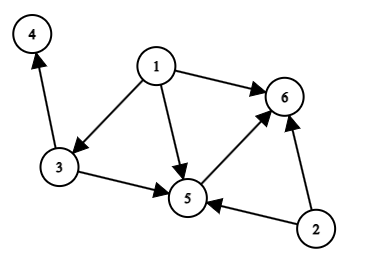
\includegraphics[scale=0.5]{./pict/exampleGraph.png}
		\caption{Graphical Example}
	\end{figure}

	\column{0.5\textwidth}
	\begin{align*}
		1 &: (3, 1) \rightarrow (5, 1) \rightarrow (6, 1)\\
		2 &: (5, 1) \rightarrow (6, 1) \\
		3 &: (4, 1) \rightarrow (5, 1) \\
		4 &: \\
		5 &: (6, 1)\\
		6 &: 
	\end{align*}			
	\centering List Representation
			
	\end{columns}
\end{frame}

\begin{frame}
	\frametitle{Implementation of Adjacency List}
	\begin{itemize}
		\item \texttt{std::vector<std::vector<std::pair<int, int>>>} to represent the adjacency list
		\begin{itemize}
			\item A pair is a specific case of a \texttt{std::tuple} with two elements.
			\item \texttt{vector[u]} is the list for \( u \in V \) 
			\item \texttt{vector[u][i].first} is the index of \( v_i \in V, (u, v_i) \in E \) 
			\item \texttt{vector[u][i].second} is the weight \( w(u, v_i) \) 	
			\item 0 indexed (\emph{yes, I know. Don't ask.})
		\end{itemize}
		\item Search whether \( (u, v) \in E \): \( O(E) \)  
		\item Space Complexity: \( O(V+E) \) 
	\end{itemize}
\end{frame}

\begin{frame}
	\frametitle{Heap based Priority Queue}
	There are many kinds of heap implementation, such as
	\begin{itemize}
		\item Binary Heap
		\item Fibonacci Heap
		\item d-ary Heap
		\item Radix Heap
	\end{itemize}
	And many more. \newline

	We shall implement \textbf{Binary Heap} 
\end{frame}

\begin{frame}
	\frametitle{Binary-Heap}
	Because of the problem specifications, we \emph{do not} concern ourselves with \textbf{construction} of heap using \texttt{BUILD-MIN-HEAP()}. Instead, the heap is \emph{maintained} through each insertion.
	\begin{itemize}
		\item \texttt{peek()}: \( O(1) \) 
		\item \texttt{extract()}: \( O(\lg{n}) \) 
		\item \texttt{decreaseKey()}: \( O(\lg{n}) \) 
		\item \texttt{insert()}: \( O(\lg{n}) \) 
		
	\end{itemize}

	\onslide<2>\begin{block}{Note}
		For heap data structure to work, we \emph{must} index from 1.	
	\end{block}
\end{frame}

\begin{frame}
	\begin{algorithm}[H]
		\caption{get index \( i \)'s parent's index}
		\begin{algorithmic}[1]
			\Function{parent}{$i$}
			\State \Return \( \lfloor \frac{ i }{ 2 }  \rfloor \) 
			\EndFunction
		\end{algorithmic}
	\end{algorithm}	

	\begin{algorithm}[H]
		\caption{get index \( i \)'s left child's index}
		\begin{algorithmic}[1]
			\Function{left}{$i$}
			\State \Return \( 2i \)  
			\EndFunction
		\end{algorithmic}
	\end{algorithm}	

	\begin{algorithm}[H]
		\caption{get index \( i \)'s right child's index}
		\begin{algorithmic}[1]
			\Function{right}{$i$}
			\State \Return \( 2i+1 \)  
			\EndFunction
		\end{algorithmic}
	\end{algorithm}	
\end{frame}

\begin{frame}
	\begin{algorithm}[H]
		\caption{min-heapify the array}
		\begin{algorithmic}[1]
			\Function{min-heapify}{$A, i$}
			\State \(l \gets \) \Call{left}{$i$}
			\State \( r \gets \) \Call{right}{$i$}
			\State \( smallest \gets i \) 
			\If{\( l \leq heapSize[A] \)}
			\State \( smallest \gets \) \Call{index-of-min}{$A[i], A[l]$}
			\EndIf
			\If{\( r \leq heapSize[A]\)}
			\State \( smallest \gets \) \Call{index-of-min}{$A[smallest], A[r]$}
			\EndIf
			\If{ \( smallest \neq i \)}
			\State \( A[i] \xleftrightarrow{} A[smallest] \)
			\State \Call{min-heapify}{$A, smallest$}
			\EndIf
			\EndFunction
		\end{algorithmic}
	\end{algorithm}	
\end{frame}

\begin{frame}
	\frametitle{Priority Queue Using Binary Heap}
	\begin{algorithm}[H]
		\caption{Extract the minimum vertex}
		\begin{algorithmic}[1]
			\Function{heap-extract-min}{$A$}
			\If{\Call{isEmpty}{$A$}}
			\State throw \textbf{error}  
			\EndIf
			\State \( min \gets A[1] \) 
			\State \( A[1] \gets A[heapSize[A]]\) 
			\State \( heapSize[A] \gets heapSize[A]-1\) 
			\State \Call{min-heapify}{$A,1$} 
			\State \Return \( min \) 
			\EndFunction
		\end{algorithmic}
	\end{algorithm}
\end{frame}

\begin{frame}
	\begin{algorithm}[H]
		\caption{decrease key value at index $i$ to $k$}
		\begin{algorithmic}[1]
			\Function{decrease-key}{$i,k$}
			\If{ \( k > A[i] \) }
			\State throw \textbf{error}  
			\EndIf
			\State \( A[i] \gets k \) 
			\While{ \( A[i] < \)  \Call{parent}{$i$} \textbf{AND} \( i > 1 \) }
			\State \( A[i] \xleftrightarrow{} \) \Call{parent}{$i$}
			\State \( i \xleftrightarrow{} \) \Call{parent}{$i$}
			\EndWhile
			\EndFunction
		\end{algorithmic}
	\end{algorithm}
\end{frame}

\begin{frame}
	\begin{algorithm}[H]
		\caption{insert vertex with index \( i \) with key \( k \)  into the queue}
		\begin{algorithmic}[1]
			\Function{insert}{$A,k$}
			\State \( heapSize[A] \gets heapSize[A]+1 \) 
			\State \( A[heapSize[A]] \gets \infty\) 
			\State \Call{decrease-key}{$A, k$}
			\EndFunction
		\end{algorithmic}
	\end{algorithm}
\end{frame}

\begin{frame}
	\frametitle{Problems}
	\begin{itemize}
		\item The heap must be able to support vertex-weight \textbf{pair} 
		\begin{itemize}
			\item It is easy to modify the data structure to include the pair
			\item Key comparison is made on the weight 
		\end{itemize}
		\item The index of the vertex-weight pair will be \textbf{shuffled} upon each \texttt{insertion()} and \texttt{extract()} 
		\begin{itemize}
			\item To prevent the \emph{loss} of information, we need a way to track their handles
			\item This is non-trivial
		\end{itemize}
	\end{itemize}
	\onslide<2> \begin{block}{Question}
		How can we track their handles?
	\end{block}
\end{frame}

\begin{frame}
	\begin{columns}
	\column{0.5\textwidth}
	\begin{figure}
		\centering
		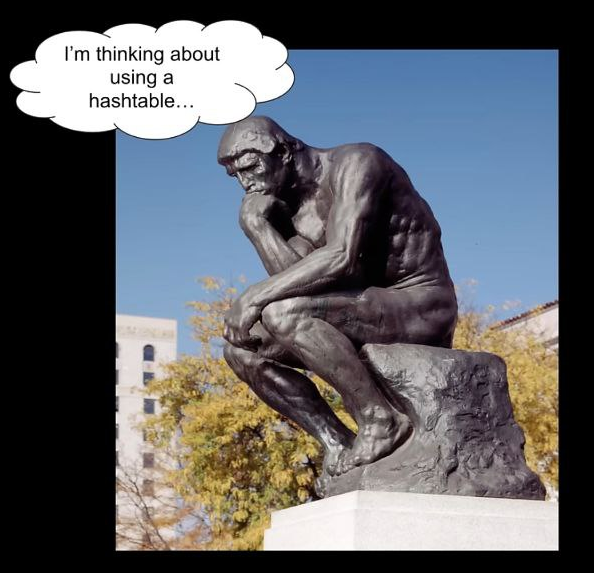
\includegraphics[scale=0.5]{./pict/secret1.png}
	\end{figure}

	\column{0.5\textwidth}
	\onslide<2>\begin{figure}
		\centering
		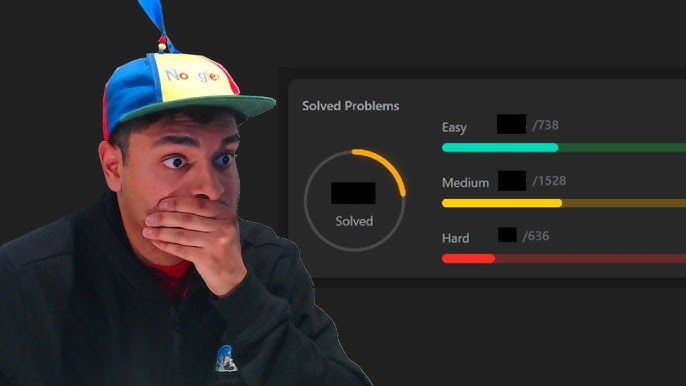
\includegraphics[scale=0.5]{pict/secret2.jpg}
		\caption{ \emph{A man and his hash map, 2024} }
	\end{figure}	
	\end{columns}
\end{frame}

\begin{frame}
	\frametitle{Implementation in C++}				
	\begin{itemize}
		\item To augment the pair, use \texttt{std::vector<pair<int, int>>} 
		\begin{itemize}
			\item \emph{Love \texttt{C++} yet?}
		\end{itemize}
		\item To track the handles, use \texttt{std::unordered\_map<int, int>} 
		\begin{itemize}
			\item \texttt{std::unordered\_map} is an associative container that contains key-value pairs with unique keys. 
			\item Search, insertion, and removal of elements have average constant-time complexity.
			\item Internally, the elements are not sorted in any particular order, but organized into buckets. 
			\item Which bucket an element is placed into depends entirely on the hash of its key.
			\item The key-value pair will be (vertex index, index in queue)
		\end{itemize}
	\end{itemize}
	\onslide<2>\begin{block}{note}
		Please refer to \texttt{JamesRobertJohns/team4projet2} 	
	\end{block}
\end{frame}

\section{Complexity Analysis and Comparison}
\begin{frame}

\end{frame}

\end{document}
